\chapter{Introduction and background} 
\label{top_of_intro}
The landscape of computational chemistry has shifted greatly over the past decade. 
The development of computational tools for chemical physics centers on approximating solutions to the Schr{\"o}dinger equation \cite{schrodinger_eqn}, whether through the development of electronic structure theory or, more indirectly, by employing classical mechanics to model molecular dynamics (MD) with force fields that have been tuned to experimental and high-accuracy quantum mechanical (QM) data.
Prior to the emergence of machine-learned methods, advancements in the field were driven by specialized approaches to solving chemical equations \cite{trp_cage_roitberg, dft_qm_mm_roitberg}, 
as well as relying on the exponential growth of hardware capabilities to simulate increasingly complex systems.
Well-established \textit{ab initio} quantum chemical methods, such as density functional theory (DFT) \cite{dft_first_paper, perspective_fifty_years_DFT, wB97X}
or coupled cluster methods \cite{coupled_cluster_first_paper, ccsd(t)_f12, dplno_ccsd(t)*},
provide close agreement with experimental methods and have long been considered the gold standard for electronic structure calculations.
Such methods carry a computational cost that scales steeply with system size---at $O(N^3)$ or greater scaling with $N$ electrons---limiting their utility in simulation of large systems or timescales relevant to many macroscopic observations. 

Computational chemistry has the persistent challenge of balancing chemical accuracy and computational cost. 
With few exceptions, approximations are necessary to determine a solution for any chemical system of interest. 
There are a variety of options for computing molecular energies but, regardless of the sophistication of the approach taken in approximating a potential energy surface (PES), there is a trade-off between the level of detail of the system and the chemical accuracy of the determined solution.
Efficient sampling techniques \cite{remd_adrian1, remd_adrian2, remd_umbrella} 
and hardware acceleration \cite{gpu_dft, gpu_quantum_chem1, gpu_quantum_chem2} 
played an essential role in mitigating some of these computational bottlenecks during the early 21st century.
The 2010s saw great strides in parallel computing, namely incorporating graphics processing units (GPUs) in chemical simulations \cite{ gpu_accelerated_AMBER, gpu_accelerated_AMBER18}
and \textit{ab initio} computations \cite{parallel_ab_initio_luehr}. 
The  complexity of larger systems make full QM calculations computationally prohibitive, necessitating hybrid approaches such as QM/MM to balance accuracy and efficiency in order to model the behavior of, for example, protein-ligand interactions \cite{dft_qm_mm_roitberg, QMtoMM_thermo_cycle}.
Some approaches to \textit{ab initio} computations increase computational efficiency by using lower-level theory with corrections to correlate with higher-accuracy methods, such as atom-centered potentials applied in the Hartree-Fock method \cite{correcting_HF_atom_centered_potentials}, though such approaches rely on hand-tuning which limits their utility as generalized potential models.
The need for a paradigm shift was clear: in order to address chemical problems ever-growing in complexity, new methodologies for efficiently computing results at quantum-levels of accuracy needed to be explored.
The work detailed here exists at this intersection, with the aim of bridging the gap between the chemical accuracy of interatomic potential models and the computational efficiency required to extend their applicability to larger and more complex systems. 

\section{The Modern Era of Computational Chemistry}
\label{sec:ML_in_chem}
The emergence of machine learning (ML) marked a transformative era of computing. 
As highlighted by Yann LeCun \cite{deep_learning_lecun}, deep learning models have excelled in many areas of data processing and, while the most popularly discussed applications are in image and natural language processing, learning models have excelled at pattern recognition and prediction in scientific data.
With vast amounts of quantum mechanical data, learning models can be trained to approximate the solutions to the Schrödinger equation with remarkable accuracy, mimicking the results of high-level QM computations.
Data-driven models have made it possible to predict molecular energies \cite{deep_tensor_NNs_schutt, prediction_errors_ml_lower_than_dft_faber, ml_atomization_energies_rupp}, 
forces \cite{interatomic_ff_ML_glielmo, md_onthefly_ml_forces_li}, 
and other properties \cite{PerSpect_ml, TensorMol}
at speeds orders of magnitude faster than computing such data with traditional QM methods on an approximate scale $O(N)$. 

Approaches to \textit{ab initio} molecular dynamics (AIMD) involve computing the interactions between nuclei and electrons, which becomes numerically demanding as the system grows larger than a few atoms.
Additionally, atomic motion must be modeled on very short timescales for dynamic calculations, leading to AIMD being an impractical approach for many chemical systems.
On the other hand, MD with classical physics treat molecules with a sort of ball-and-spring representation, where atoms oscillate around equilibrium bonding distances with neighboring, bonded atoms.
This approach to chemical simulations has long been the standard for studying macromolecular systems, notably biomolecules and polymers.
However, many systems of biological relevance include changes to bonding (\textit{e.g.}, reactions taking place in protein active sites), which force fields are unable to model due to explicitly defining the molecular topology.

Machine learning offers a route to circumvent this computational bottleneck by learning from precomputed data: models trained on small-scale, high-quality QM data have been shown to capture the physics of complex molecular systems and scale this behavior up to large-scale systems \cite{ml_mm_largescale}. 
The use of machine-learned potential energy surfaces (ML-PES) has been particularly advantageous for using MD simulations to explore complex chemical potential energy landscapes, which were previously inaccessible due to these computational constraints. 
The strength of ML-PES lies in their capability to balance chemical accuracy with computational cost, allowing for simulations of QM-realm behavior to be modeled at force field computational efficiency. 
Further, ML-PES differ from classical force fields in their ability to model changes in bonding \cite{reactive_nnp_behler, yinuo_reactive_MLPs}, whereas traditional force field models parameterize bonds and explicitly connect atoms in the system topology.
Advances in ML-PES advance the scope of computational chemistry by providing insights into chemical phenomena that were previously out of reach.
The use of ML-PES is not flawless, however, as machine-learned models can very easily migrate into regions of chemical space that they are ill-equipped to handle, \textit{i.e.}, chemical behavior outside of the data the model was trained on.
To minimize this, there are a few important considerations when implementing a machine-learned interatomic model: atomic representation, model architecture, and the quality and availability of training data.


\subsection{Atomic Representation}
\label{subsec:ML_atomic_representation}
In order to train learning models, or use any computational method for chemical systems, one must consider the molecular or atomic representation which defines the system. 
This is especially important in atomistic ML models, where the atomic representation is the input which the predictive algorithm uses to estimate a property of the system.
Many viable pre-defined atomic descriptors have been reported in the literature \cite{atom_centered_symmetry_function_behler, PIP_NN, DeePMD, esders_atomic_NNP}, which focus on identifying the local chemical environment surrounding each atom. 
Some applications further refine these representations with learnable descriptors, which can fit to more complex data on-the-fly as needed \cite{wACSF, SchNet, PhysNet, AIMNet_NSE, NequIP, interatomic_descriptors_kabylda}.
The most popular of these approaches for describing local atomic environments was developed by Behler and Parrinello \cite{atom_centered_symmetry_function_behler}, and further modified to better fit to training data \cite{TensorMol, ani-1}.
Behler-Parrinello (BP) symmetry functions were among the earliest successes in generalized machine-learned interatomic potential models \cite{behler_parrinello}, demonstrating the capabilities of ML-PES to capture complex, many-body interactions within chemical systems.
An example of modified BP atom-centered symmetry functions \cite{ani-1}, computed for each atom to identify neighboring species within a pre-defined cutoff radius, are shown in Equations \ref{eq:smooth_cutoff}, \ref{eq:radial_symmetry_function}, and \ref{eq:angular_symmetry_function}. 
The first of these equations is the cutoff function, $f_C$, used to smoothly fade out atoms near the boundary of the local atomic environment defined by $R_C$. Here, $R_{ij}$ is the Euclidean distance between two atoms $i$ and $j$ and $\epsilon = 10^{-10}$ to prevent division by zero in the case of an atom at exactly the cutoff radius. 

\begin{equation}
f_C(R_{ij}) = 
\begin{cases} 
\exp \left(1 - \frac{1}{1 - \left(\frac{R_{ij}}{R_c}\right)^{2} + \epsilon} \right) & \text{for } R_{ij} \leq R_C \\
0.0 & \text{for } R_{ij} > R_C 
\end{cases}
\label{eq:smooth_cutoff}
\end{equation}

Within the specified cutoff radius, modified BP symmetry functions are comprised of two components. 
The first of these components is a radial symmetry function $G^{A_{\text{mod}}}_m$, which probes outwards from a central atom to determine the distances to all neighboring atoms with a series of Gaussian functions of width $\eta$ centered at $R_s$.

\begin{equation}
  G_{m}^{\text{R}} = \sum_{j \neq i}^{\text{all atoms}} \mathrm{e}^{-\eta (R_{ij} - R_{s})^2} f_{C}(R_{ij})
  \label{eq:radial_symmetry_function}
\end{equation}

The second equation used in constructing BP-type symmetry functions is the angular component $G^{_{\text{mod}}}_m$, which uses Gaussian functions---similar to $G^{A_{\text{mod}}}_m$, despite a more complex formulation---to compute three-body angular factors surrounding atom $i$ and all possible pairs $j$ and $k$. 
Here, $R_{ij}$ and $R_{ik}$ are pairwise distances between the central atom and each of the neighboring atoms. 
Two new parameters, $\theta_{s}$ and $\xi$, are used to define the angular environment by controlling the angle and width of the Gaussian probe respectively. 
$\theta_{ijk}$ represents the angle between $i,j,k$, and the parameters $\eta$, $R_s$, and $f_C$ serve the same purpose as in Eqn. \ref{eq:radial_symmetry_function}.

\begin{equation}
    G^{A_{\text{mod}}}_m = 2^{1-\xi} \sum_{j,k \neq i}^{\text{all atoms}} \left( 1 + \cos(\theta_{ijk} - \theta_s) \right)^\xi \exp \left[ -\eta \left( \frac{R_{ij} + R_{ik}}{2} - R_s \right)^2 \right] f_C(R_{ij}) f_C(R_{ik})
    \label{eq:angular_symmetry_function}
\end{equation}

With a well-defined constructor, such as atom-centered symmetry functions, one must consider an encoding which preserves key structural and chemical information while maintaining rotational, translational, and permutational invariance.
This encoding, often represented as a vector of descriptors, serves as the input to a learning model, determining its ability to distinguish variations in chemical environments and generalize across diverse molecular systems.
The utility of atom-centered symmetry functions and atomic descriptors is further explored in section \ref{subsec:AEV}.


\subsection{Model Architecture}
\label{subsec:ML_model_architecture}

The representation of atomic environments is an important facet of machine-learned interatomic potential models, but the predictive power of a learning model is determined by the choice of architecture. 
A variety of ML model architectures have been explored in the literature to address challenges in chemical simulation, including: 
graph neural networks (GNN) \cite{gnn_property_prediction1, gnn_property_prediction2}, 
Gaussian process regression models \cite{gaussian_process_regression1,gaussian_process_regression2}, 
gradient-domain machine learning \cite{ml_energy_conserving_ff_chmiela}, 
and deep artificial neural networks (ANN) \cite{pes_fitted_by_NN_handley, ab_initio_pes_using_ml_lu, ml_pes_jiang}. 
Of these, some models---such as Gaussian process regression models---prioritize interpretability and precision of predictions, while others, particularly ANN potential models, emphasize the scalability and accuracy of high-dimensional potential energy landscapes in diverse systems.

Historically, neural network models were seen as an excellent tool for specialized approaches to understanding specific chemical systems \cite{specialized_nnp1, specialized_nnp2}, but breakthroughs in flexible, generalizable models have shifted the focus to building models which can predict properties of any molecular system within the realm of the data on which it was trained \cite{ani-1, behler_parrinello}. 
Deep neural networks are a mathematical framework involving a series of nodes assembled in layers. 
An example of a small but typical deep neural network is given in \ref{fig:nn_arch}, created using NN-SVG \cite{NN_SVG}.

\begin{figure}[!h]
    \centering
    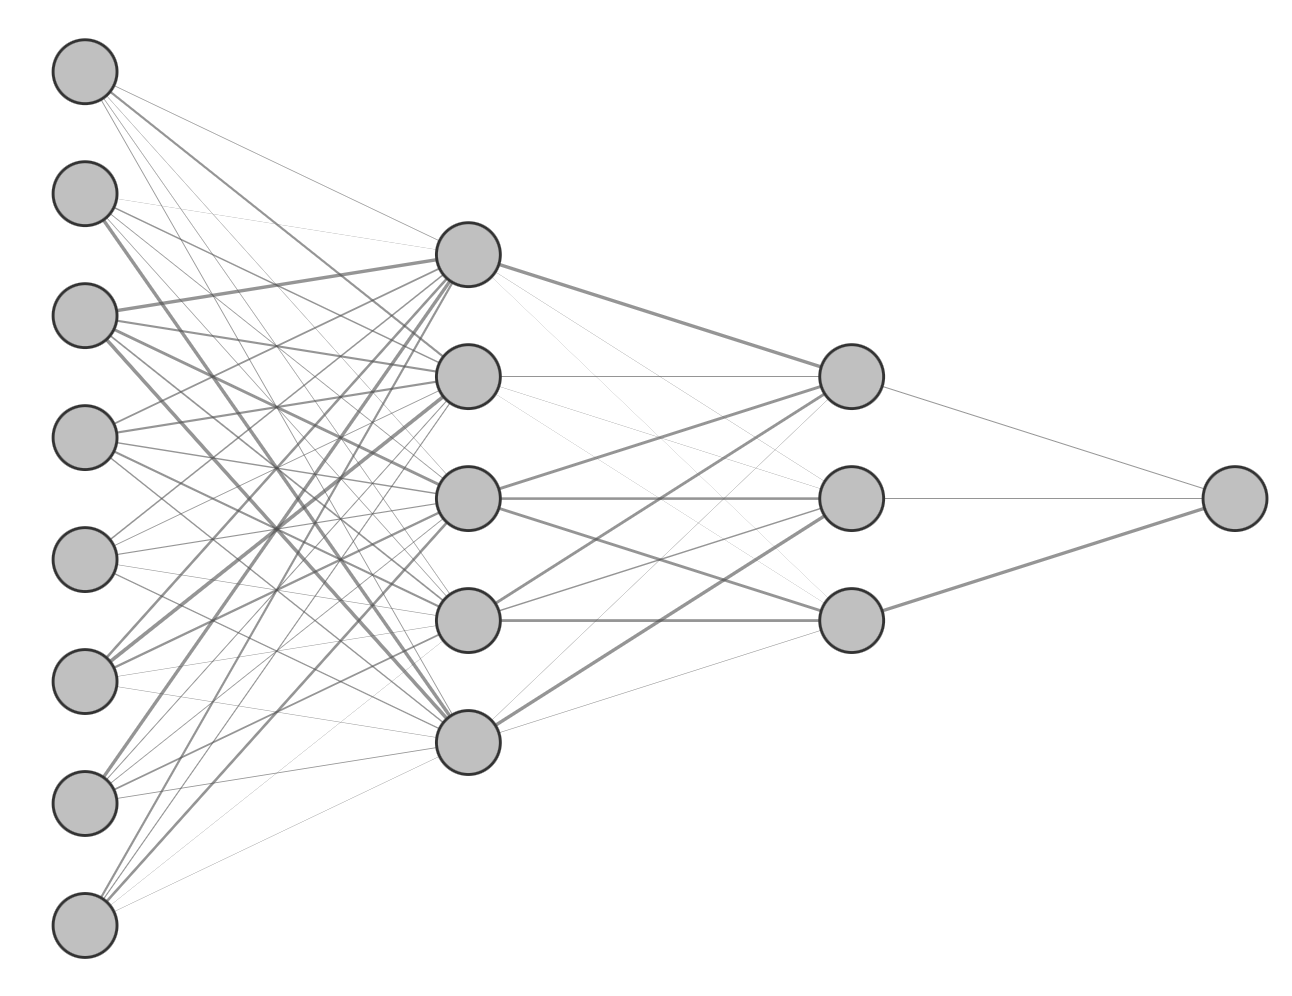
\includegraphics[width=0.8\linewidth]{Images/nn_arch.png}
    \caption[Example structure of a deep neural network]{Example structure of a deep neural network architecture comprised of an input layer, two hidden layers, and an output layer. The weights on each connection are represented by the intensity of the line the nodes.}
    \label{fig:nn_arch}
\end{figure}

Neural networks are typically funnel-shaped, reducing high-dimensional data to a lower dimensional representation as information is passed through the layers. 
The nodes in a single layer are connected to each node in the adjacent layers via weights, which are iteratively updated in order to reproduce the behavior of the data pushed through the network throughout the training process. 
The nodes receive a signal from either the input (at the input layer) or from connected nodes, which varies in intensity depending on the weight of the connection.
Higher-weighted connections have a stronger influence over the activation of the subsequently connected node.
The signal input to a node passes through a nonlinear activation function, which transforms the weighted-sum of all inputs from the previous layer into some output value.

The connections between neural network nodes can be expressed with a simple mathematical formulation, shown in Eqn. \ref{eq:nn_eqn}, where the output value $y$ is obtained from the weighted (by $w_i$) sum of inputs $x_i$, which is often (though not always) adjusted with a bias value $b$. 

\begin{equation}
y = \sum_{i}^{n} (w_i x_i) + b
\label{eq:nn_eqn}
\end{equation}

For the input and hidden layers, this value is passed onto the next layer, where the same operation takes place.
The output layer produces a prediction value for the given input, though sometimes the output value undergoes one last transformation to shift into the range of values expected by the data used in training.

The size and shape of neural networks greatly influence their ability to capture complex behavior in chemical systems.
Shallow networks with few neurons are excellent tools for learning the patterns in low-dimensional data, but many interacting chemical species require an increasingly broad and deep network size to learn the landscape of possible chemical interactions.
However, larger network sizes are not necessarily better: excessively deep neural networks are more costly to train and increase risks of overfitting; networks with too many neurons expect higher-dimensional behavior than the interactions captured in the training data.
Balancing the size of networks with the complexity and scope of the data used in training is vital for designing model architectures that achieve the accuracy and efficiency that has become synonymous with interatomic neural network potential (NNP) models. 

Supervised training of ML models involves iteratively passing data through the networks and asking the model to predict a desired property of the data.
This output prediction is compared to a reference value, as training data is labeled, and the predictive error is computed to weigh in the loss, or cost, function which determines how much the weights need to update in order to better capture the behavior represented in the training data. 
In interatomic potential models, at least within the scope of the work presented here, the labeled data is \textit{ab initio} computations of molecular energy and the forces acting upon atoms within a molecular conformation.
The weights are updated via a fine-tuning process known as backpropagation, which uses a stochastic gradient descent optimizer such as Adam \cite{adam_optim} to change the weights based on the gradients of the loss function at each training iteration. 
Another important hyperparameter used in training neural network models is the learning rate, which controls the step size in weight adjustments.
Learning rate plays an important role in reaching convergence when training: a large value can prevent the model from reaching stable predictions, while low learning rates can slow the training process and lead to increased computational costs to reach converged behavior.

Achieving broad generalizability of chemical systems requires large quantities of carefully crafted training data.
Training efficiency can be increased by batching data into smaller segments, which helps the model learn the relationship between molecular structure and the desired predicted properties without specifically memorizing individual pieces of the training data, which is referred to as overfitting.
The choice of training data greatly impacts the ability of a model to extrapolate between conformational and configurational relationships observed in training with the novel use cases encountered in inference. 
Without representing generalized behavior in the training data, a model will be unable to represent generalizable performance and applicability.
Section \ref{subsec:Data quality and availability} explores the importance of comprehensive training data in the development of ML models.

\subsection{Data Quality and Availability}
\label{subsec:Data quality and availability}

Statistical learning models are bounded in accuracy by the quality and quantity of data used in training. 
Many applications of machine learning, such as computer vision, have an abundance of data available for training a model to artificially reproduce \cite{deep_learning_lecun}. 
In computational chemistry, however, the object is largely to explore and model behavior that is not understood well, meaning the data which describes phenomena of interest is often sparce and must be generated specifically \cite{ml_energy_conserving_ff_chmiela, pes_fitted_by_NN_handley, ab_initio_pes_using_ml_lu, protein_ff_fragmentation_nn_wang, PES_gasphase} for use in training a learning model to reproduce the physical behavior of systems of interest. 

Data quality is an abstract and difficult to define concept.
In the context of chemical simulation, high-quality data encompasses the accuracy of the underlying physics utilized, as well as the diversity of chemical environments modeled.
Ideally, a properly constructed ML interatomic potential model can learn to represent any dataset, though in practice this is difficult to achieve.
Chemical space is immense, and could be considered practically infinite; up to $10^{60}$ organic molecules \cite{chemical_space} fall into the space loosely defined by Lipinski's rule of five \cite{lipinski} for druglike molecules.
Curating a dataset which represents all possible behavior even limited to this subsection of chemical space is challenging due to the vast possibilities in configurational and conformational diversity.

Poor-quality data can lead to systematic errors in learned potential energy landscapes, reducing the reliability and transferability of ML potential models.
Deficiencies in data quality arise from many factors including, but not limited to: the approximations made in one's choice of \textit{ab initio} theory, which become a source of error in computed molecular energy and atomic forces; limited sampling of conformational and configurational chemical space, restricting the exposure of varied chemical environments to the model; and biases in data selection, which can lead to an overrepresentation of chemical motifs and skew predictive capabilities or lead to overtraining.
Addressing these challenges requires careful dataset curation to capture the accuracy of the underlying physics represented in training data with broad coverage of relevant chemical environments.

The accuracy of reference data labels is vital to the fidelity of an ML model. 
In NNP models trained on \textit{ab initio} molecular energy computations this corresponds to the level of quantum theory utilized in generating the training data, such as DFT \cite{dft_first_paper} or coupled-cluster \cite{coupled_cluster_first_paper} methods.
Lower-level methods introduce approximation errors that will be learned by the model, whereas higher-level, more chemically accurate methods are too computationally prohibitive to apply to large systems or for generating vast quantities of data.
One possible solution to this trade-off is the use of transfer learning, where the base-level physics are learned from lower-level theory, and the model is later fine tuned with a small subset of data produced by more computationally expensive methods.
Applications of transfer learning are discussed in greater detail in Subsection \ref{subsec:ANI_datasets}.

Beyond the accuracy of reference data, diversity plays an integral role in the robustness of a model.
Datasets limited to a narrow region of chemical space---\textit{e.g.}, only sampling equilibrium geometries or from a small subset of chemical species---will result in less generalizable inference performance when encountering unseen molecular structures, despite reporting low errors during testing and validation.
Conformational sampling of molecular structures in off-equilibrium geometries is relatively straightforward, requiring the identification of regions of chemical space where model uncertainty is highest and distorting bond angles and distances around those regions.
This type of sampling is widely used in active learning approaches to generating data that fills gaps in ML model understanding.
Sampling new molecular configurations via active learning is more involved; after identifying high-uncertainty predictions, new structures must be strategically selected to include underrepresented chemical motifs.

In addition to the quality of data used in building training sets, one must consider the availability of that data.
For ML interatomic potentials trained on QM energies, data availability pertains to the feasibility of generating large datasets of molecular properties, where molecular size and atomic complexity are the limiting factors to computing vast amounts of data at sophisticated levels of theory.
Public datasets of first-principles calculations \cite{qm9, qm40} help to mitigate this limitation, though these are the result of ongoing efforts to expand the availability of high-accuracy quantum chemical data.

This consideration is further applicable to tools used to predict experimental results such as NMR chemical shifts \cite{shiftx, legolas} from structural geometries.
For example, the neuraL nEtwork enGine fOr caLculating chemicAl Shifts (LEGOLAS) \cite{legolas} gives rapid, accurate predictions of NMR chemical shifts for backbone atoms of proteins, making it a useful approach to structure elucidation and validation in molecular biology.
However, like all ML models, its performance is intrinsically tied to the quality and availability of training data.
LEGOLAS exhibits high accuracy for well-represented chemical environments, but shows poor inference performance on atoms in residues with sparse (or high-uncertainty) training data.
This highlights a fundamental obstacle in machine-learned predictions of chemical systems: achieving reliable generalization requires datasets that comprehensively capture the vastness of chemical space that could be encountered in real-world applications.

The interplay between data availability and quality with the transferability of a fully-trained ML model highlights the importance of dataset curation for developing a generalized ML interatomic potential model.
The broader implications of data limitations extend to various chemical applications, from force field development, modeling of chemical reactions, and prediction of molecular properties.
The ability of ML models to generalize behavior across the complexity of chemical space remains a challenge, though exemplary models have shown success in producing high-accuracy predictions.
One such example is explored in Section \ref{sec:ANI_intro}, which will remain the focus of the work presented in the subsequent chapters, and serves as a case study for understanding how neural network potentials can be applied to streamlining energy calculations at quantum-levels of accuracy, as well as the simulation of reactive chemical environments.


\section{The Artificial NeurAl networK engINe for Molecular Energies: ANI}
\label{sec:ANI_intro}

Within the realm of machine learning in chemistry and neural network potentials, the Artificial NeurAl networK engINe for Molecular Energies (ANAKIN-ME, commonly referred to as ANI) \cite{ani-1} was a landmark development in potential energy surface predictions.
Building on the foundations set by earlier NNP models, such as HDNN \cite{behler_parrinello} by Behler and Parrinello, ANI-1 used an atom-specific neural network architecture to predict molecular energies with chemical accuracy comparable to density functional theory at a speedup of approximately $10^6$.
Implemented in a C++ and CUDA program called NeuroChem, ANI-1 was trained on a dataset \cite{ani-1_dataset} of 17.2 million small organic molecules containing only hydrogen, carbon, nitrogen, and oxygen atoms. 
Despite the training set containing only up to 8 heavy (non-hydrogen) atoms, the model performed well on test sets of 10-24 atoms---within 1 kcal/mol of the DFT reference energy for near-equilibrium structures \cite{ani-1}.
ANI-1x \cite{ani-1x} and 1ccx \cite{ani-1ccx} were introduced as an improvement over ANI-1 by using smaller, more carefully crafted datasets to achieve greater accuracy, generalization, and scalability; the cultivation of these datasets is explored in Subsection \ref{subsec:ANI_datasets}.
Figure \ref{fig:accuracy-cost} qualitatively demonstrates how the various published ANI models perform against routinely applied methods in computational chemistry, showcasing that ANI is capable of predicting molecular energies with first-principles levels of accuracy at approximately the same cost as force field methods.

\begin{figure}[!ht]
    \centering
    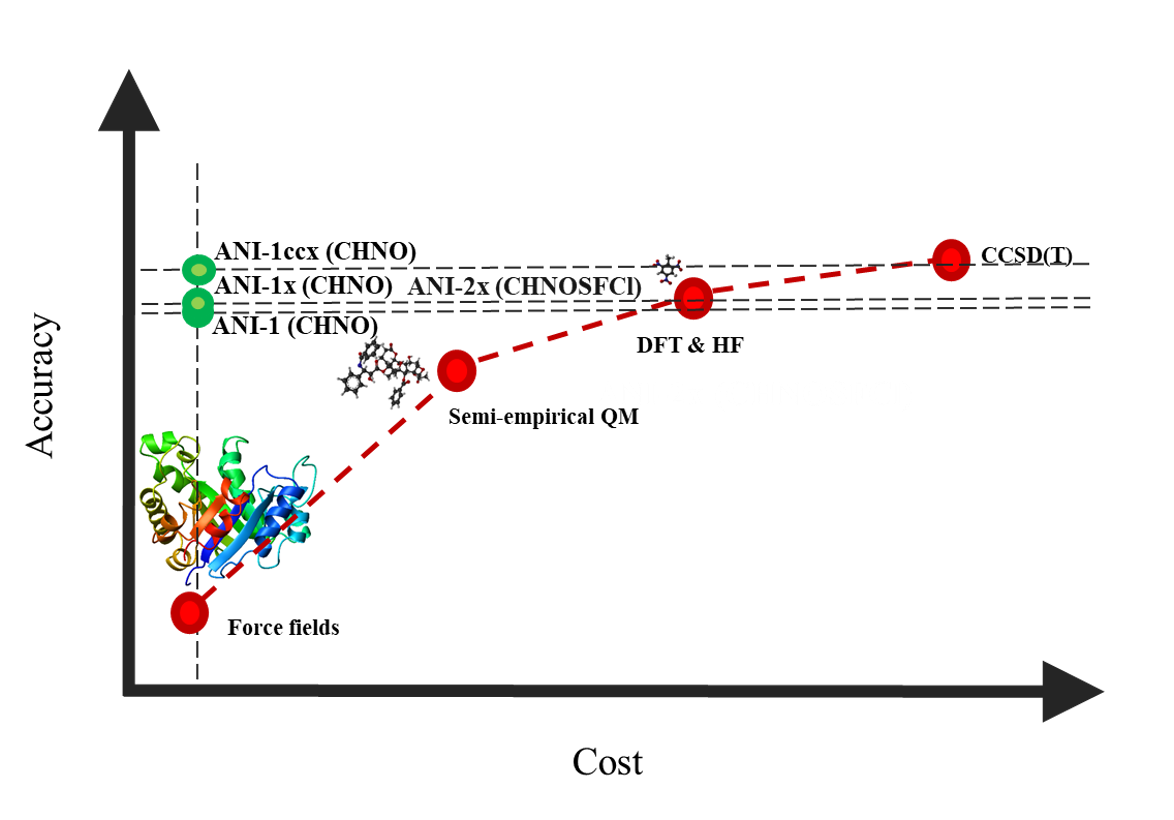
\includegraphics[width=1\linewidth]{Images/accuracy-cost.png}
    \caption[Approximate scaling of compute time versus chemical accuracy]{
    Approximate scaling of compute time versus chemical accuracy in various computational chemistry methods. Neural network potential models in the TorchANI package compute energies at DFT (or greater) levels of accuracy, at a cost similar to that of force fields.
    }
    \label{fig:accuracy-cost}
\end{figure}

The ANI methodology was further extended to sulfur, fluorine, and chlorine with the release of ANI-2x \cite{ani-2x, 2x_dataset} and implemented in Python using the PyTorch library \cite{pytorch} in the TorchANI package \cite{torchani}.
With these advancements, and adaptations to traditional QM/MM embedding approaches for boundary atoms, the ANI-2x potentials have been applied to hybrid ML/MM schemes \cite{ml_mm_galvelis, ml_mm_santi_y_jonny1, ml_mm_santi_y_jonny2}.
ANI-style networks have also proven useful in rapid, parallelized predictions of NMR chemical shift ($\delta$) values for protein backbones \cite{legolas, torchani}, particularly in their application in molecular dynamics simulations.
Reactive potentials such as ANI-1xnr \cite{ani-1xnr} further extend the predictive capabilities of ANI neural network potentials; refer to \ref{subsec:ANI_datasets} for details on the dataset used in training this reactive potential.

To better understand the ANAKIN-ME methodology, we must look more closely at a few aspects: the descriptor, Atomic Environment Vectors; the structure of ANI neural networks; and the datasets used for training, validating, and testing ANI models.

\subsection{The Atomic Environment Vector}
\label{subsec:AEV}

A fundamental component of the predictive accuracy of ANI models is the construction of the Atomic Environment Vector (AEV) \cite{ani-1}, which provides a systematic approach to encoding local atomic interactions.
Using the modified BP symmetry functions \cite{behler_parrinello} given in Equations \ref{eq:radial_symmetry_function} and \ref{eq:angular_symmetry_function} within a specified cutoff radius---5.1 \angstrom for the radial component and 3.5 \angstrom for the angular component---an atom-centered representation of the local chemical environment is constructed into a fixed-length vector.
An example of the angular AEV radius is given in Figure \ref{fig:aev_radius}.
The leftmost image shows the molecule used in the example, while the middle image is a demonstration of the cutoff radius, and the rightmost image shows how atoms outside of this radius are not seen by the atom an AEV is being constructed for.

\begin{figure}[h!]
    \centering
    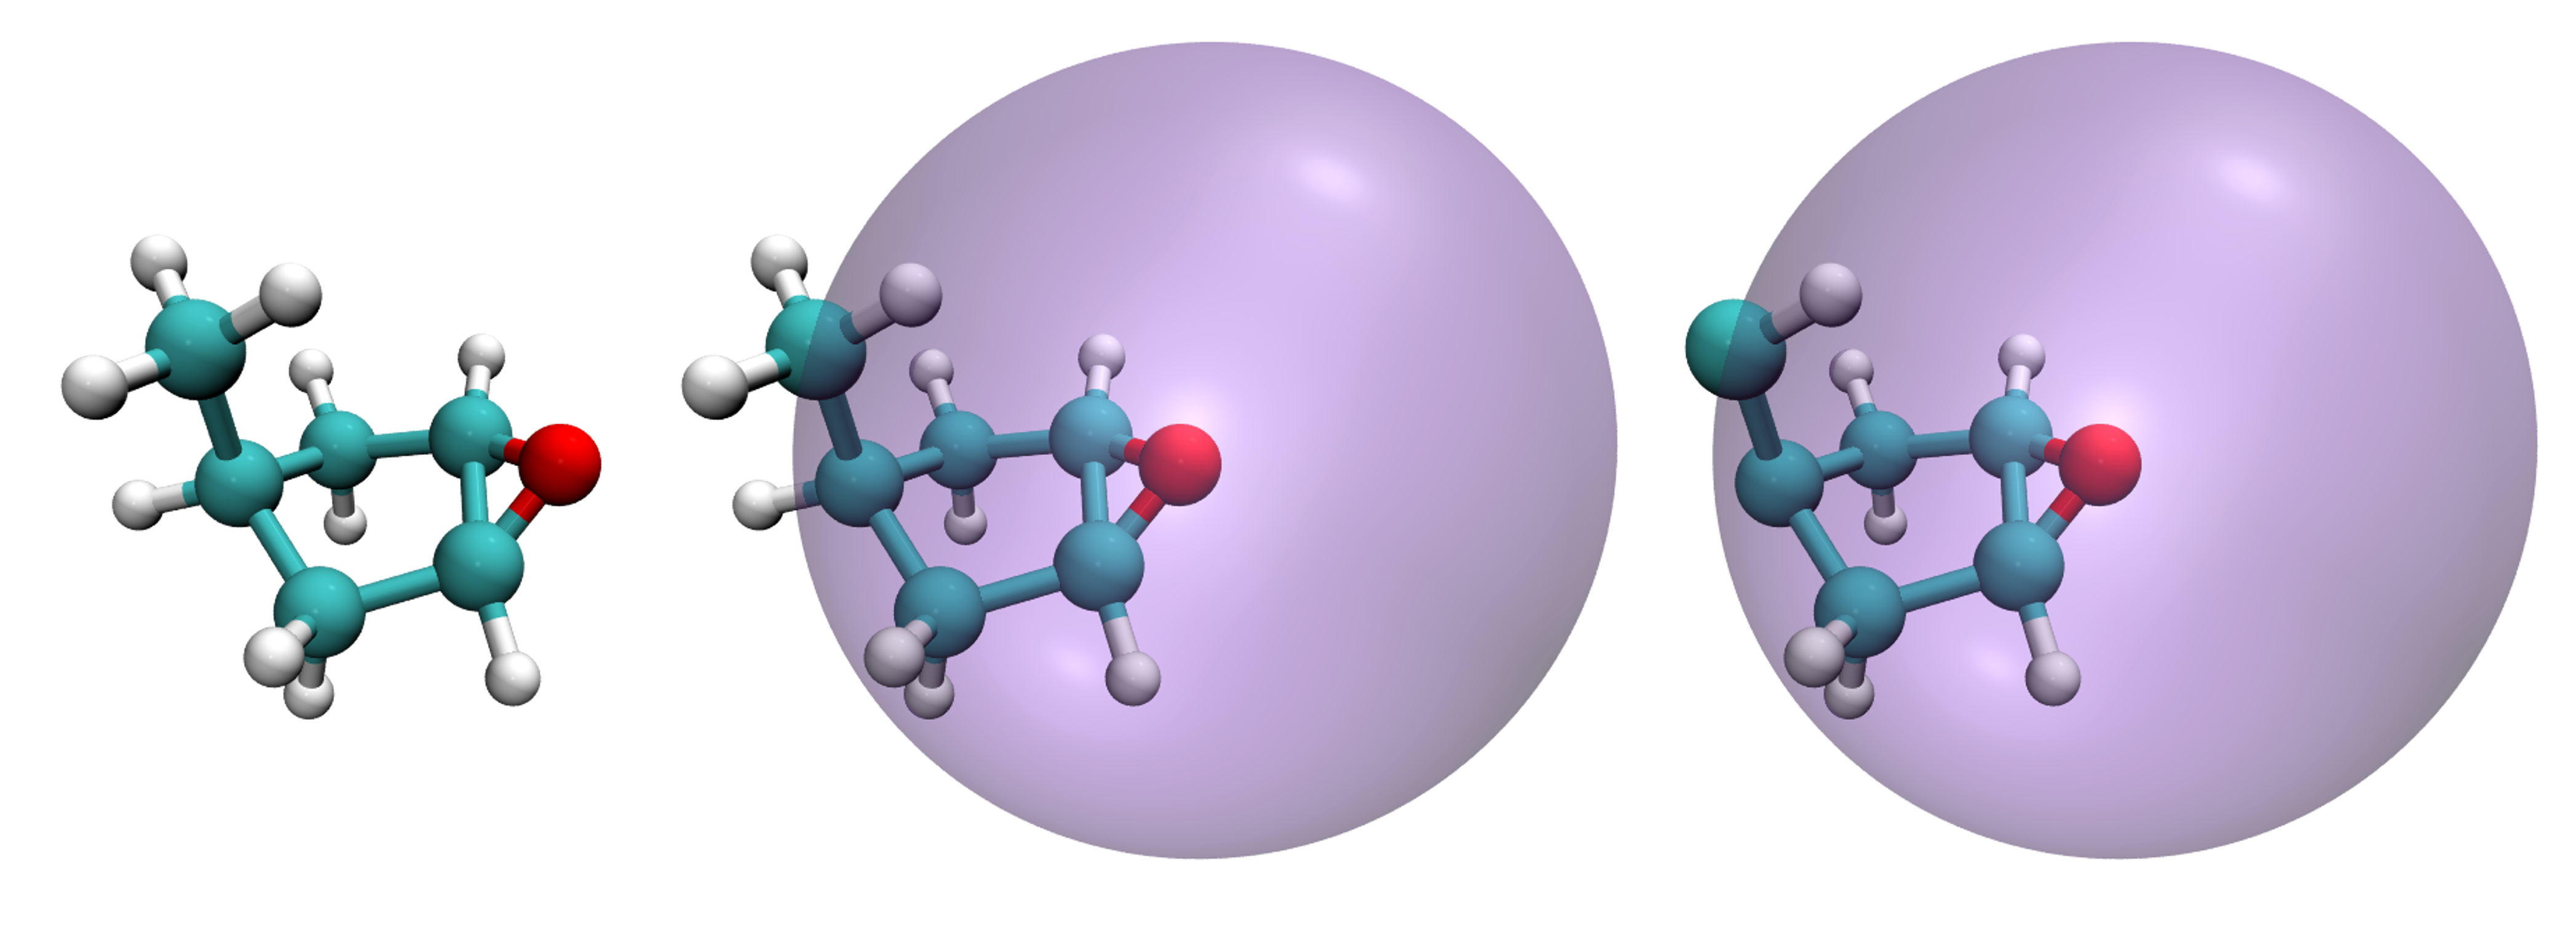
\includegraphics[width=1\linewidth]{Images/aev_radius/aev_radius_combined.png}
    \caption[Demonstration of AEV angular cutoff radius.]{Angular cutoff radius for the oxygen in C$_6$H$_{10}$O. Note that three hydrogen atoms fall outside of the cutoff radius, making them effectively invisible to the oxygen atom.}
    \label{fig:aev_radius}
\end{figure}

As described in Subsection \ref{subsec:ML_atomic_representation}, the radial component embeds two-body interactions based on distances between atoms, while the angular component embeds three-body interactions for all possible pairs of neighboring atoms.
This representation is designed to be rotationally, translationally, and permutationally invariant, meaning that chemically equivalent atoms are treated consistently regardless of their spatial orientation or ordering within the molecular structure.
Unlike Behler-Parrinello symmetry functions, the AEV computer utilized in the ANI methodology incorporates information about the atom types (elements) encoded in the atomic representation, which in turn yields lower-error predictions on multi-molecule training sets and permits better transferability \cite{ani-1}.
Figure \ref{fig:aev_construction} is a schematic representation of the AEV construction. 

\begin{figure}[hb]
    \centering
    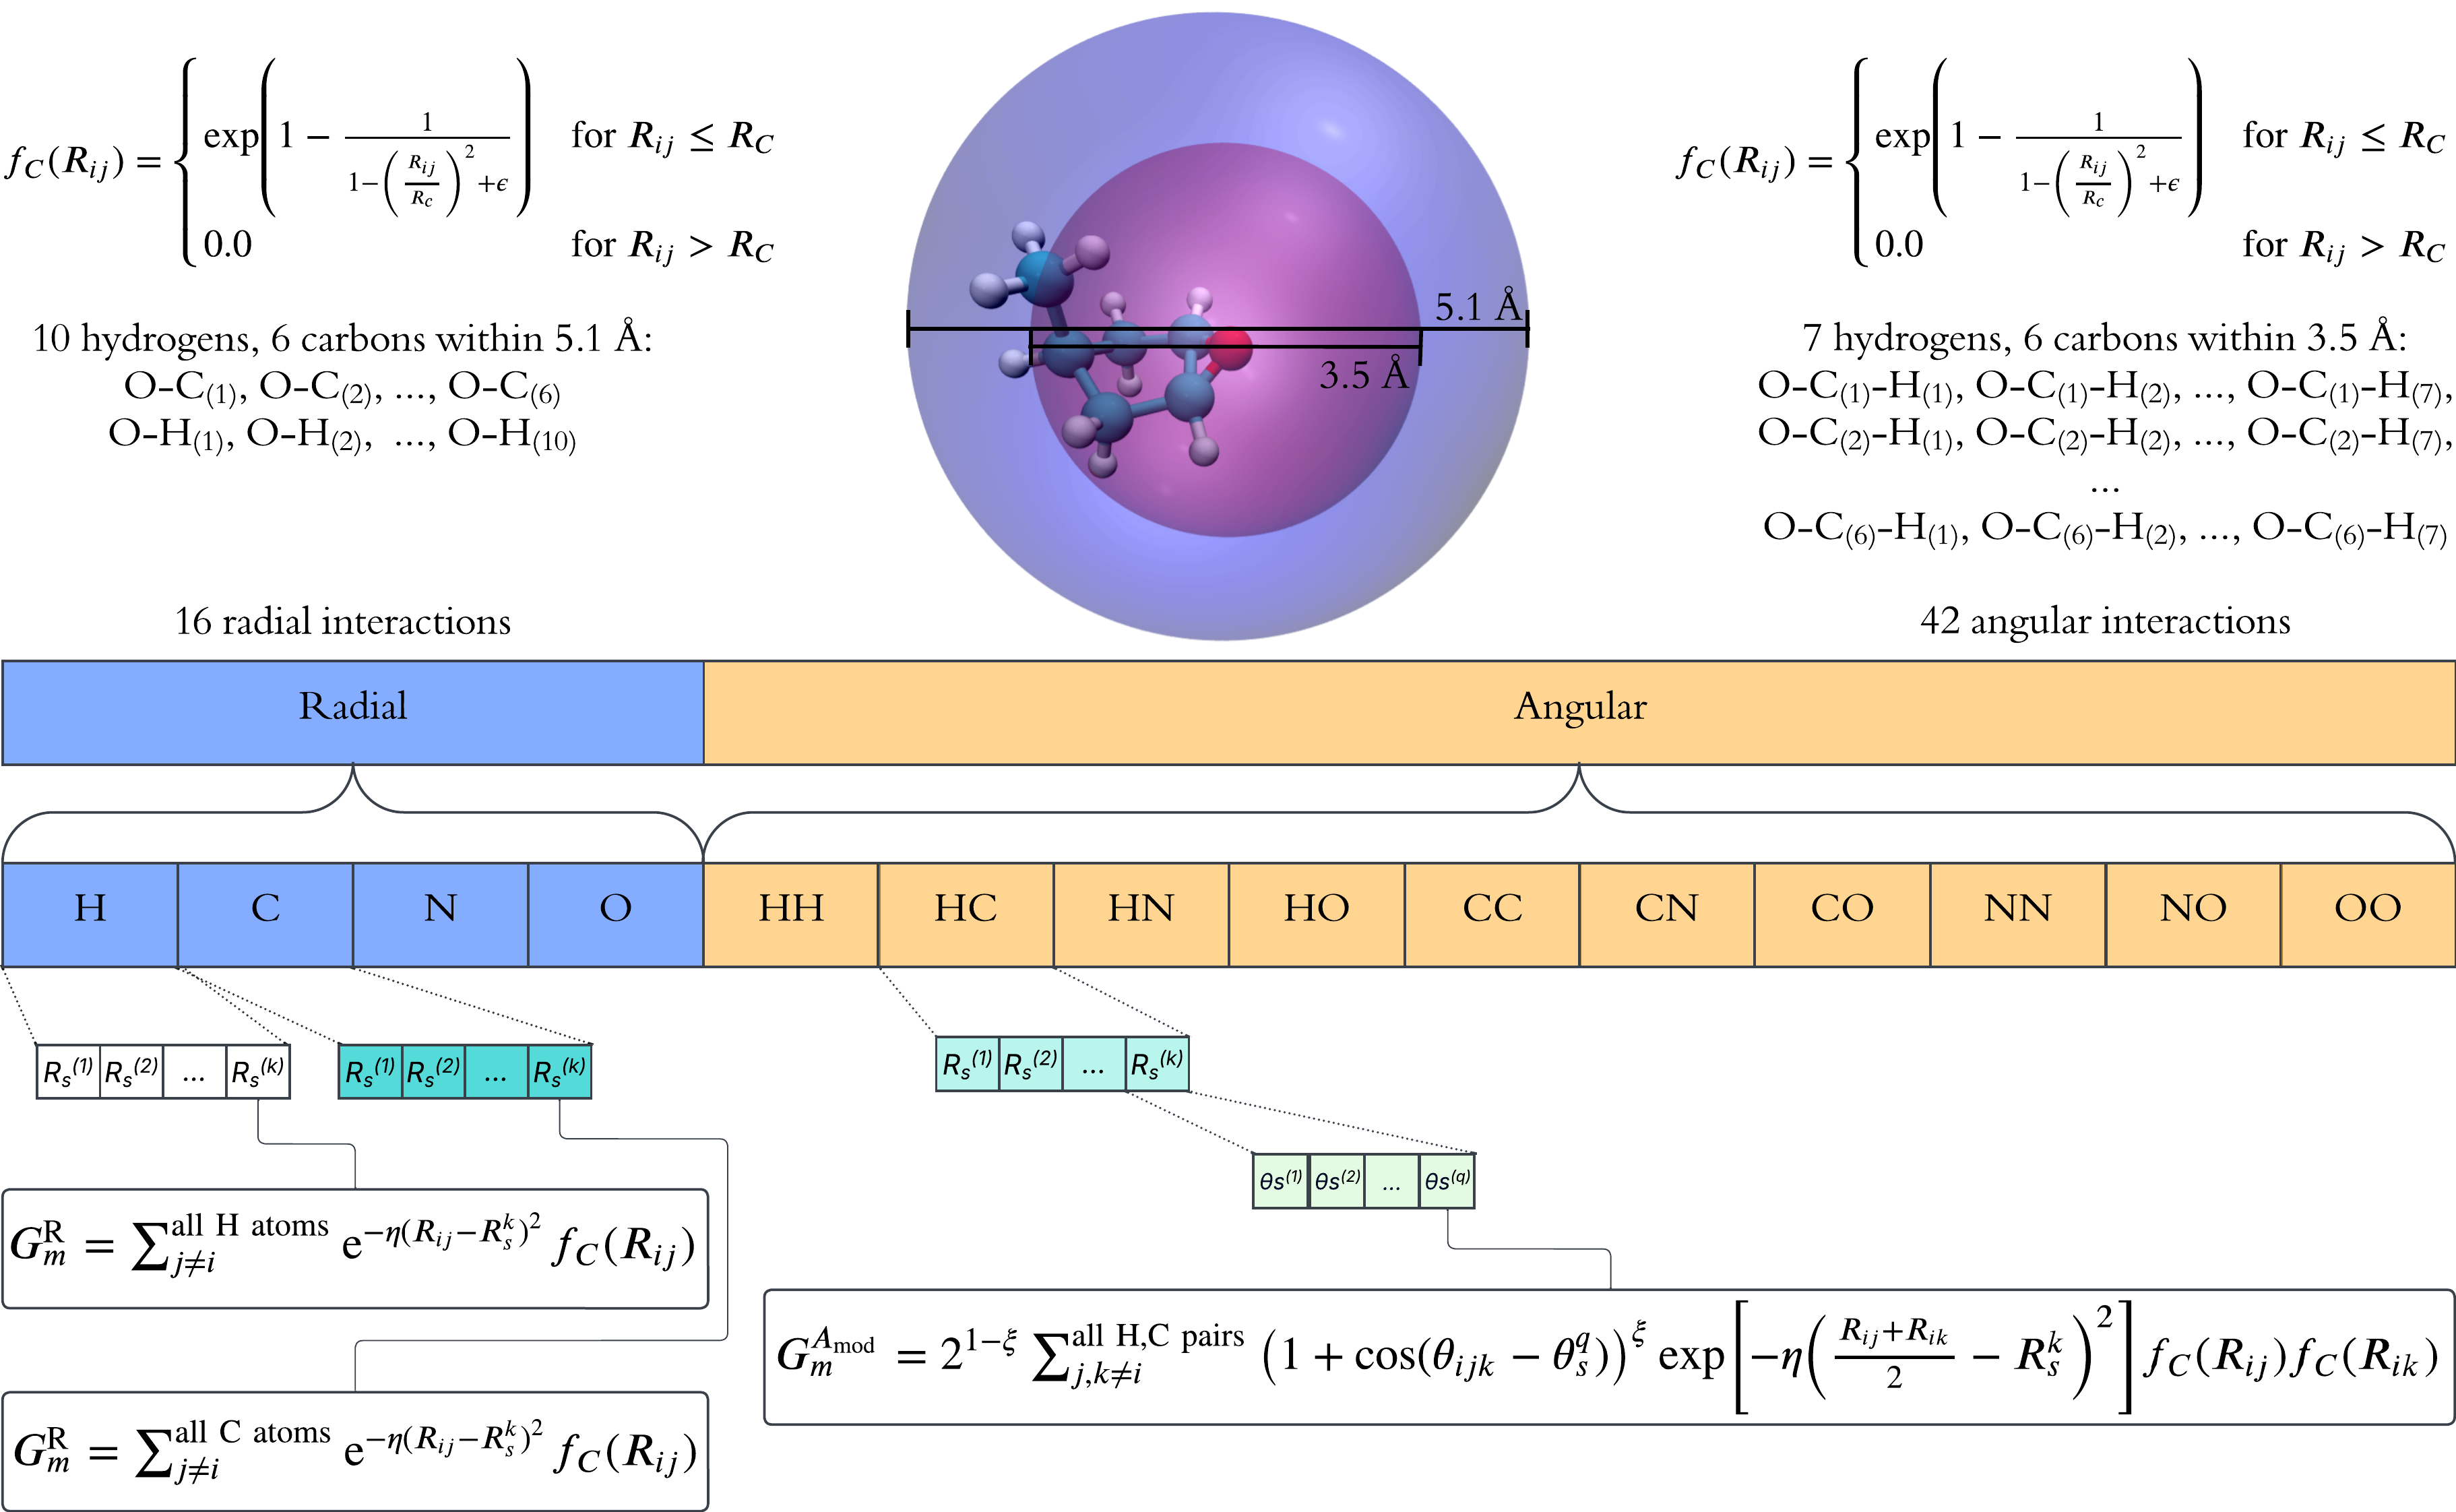
\includegraphics[width=1\linewidth]{Images/aev_radius/AEV_construction.png}
    \caption[Schematic of atomic environment vector construction]{Example of the terms in an AEV for the lone oxygen in the C$_6$H$_{10}$O molecule used in Fig. \ref{fig:aev_radius}.}
    \label{fig:aev_construction}
\end{figure}

During training and inference, AEVs serve as the inputs to element-specific neural networks, where they are used to predict the contribution of each atom to the total molecular energy.
This relationship is explored in detail in Subsection \ref{subsec:total_E_sum_AEs}.
The scalability of ANI predictions is due to this representation of local atomic environments and, though it neglects long-range interactions, does well to predict molecular energies for systems much larger than those included in the training sets \cite{ani-1x, ani-2x}.

The use of a robust descriptor is vital to creating a generalized representation of chemical environments, and serves as the basis for modeling chemical behavior.
However, a robust descriptor is just one component of a successful ML model; the neural network architecture built around these descriptors enable efficient learning of the chemical relationships in QM data.
The following section explores the architecture of ANI models, and how the fixed-length AEV is used as an input to produce predictions of molecular energy.


\subsection{ANI Model Architecture}
\label{subsec:ANI_model_arch}

The ANI models use a modular neural network architecture, where each unique atom type employs a species-specific feedforward network to learn the relationships between local atomic environment and the contribution of each atom in the system to the total molecular energy.
This energy decomposition makes it possible for ANI to efficiently scale to systems outside of the scope of the training data. 
Each of the species-specific networks are similar in structure, containing the same number of neurons in the input layer (equal to the AEV size) but employ different hidden layer shapes due to variations in atomic bonding and dataset composition.

The hidden layers transform the input AEV into a high-dimensional latent feature space where patterns in atomic interactions and energy can be learned effectively.
The input signal undergoes dimensional reduction with each hidden layer, becoming more abstract to capture nonlinear, chemically relevant patterns in the data input to the network. 
This funnel-shaped network structure, combined with the robust descriptor detailed in Subsection \ref{subsec:AEV}, are key in the ability of ANI models to make generalized predictions beyond the training dataset.

Neural networks are highly flexible, and can learn to predict properties of unseen data based on trends in the, often, very high-dimensional data used in training.
Supervised training, as mentioned in Subsection \ref{subsec:ML_model_architecture}, is the iterative optimization process of updating the weights connecting nodes in neural networks to minimize the error between predicted and labeled data.
This optimization is based on the output of a loss function.
For ANI models, the most basic chemical property trained to is the total molecular energy.
The predictive error of an ANI model is minimized in training using a mean squared error loss function that quantifies the difference between predicted molecular energy and the QM reference values.
An example of the energy loss function utilized in training a typical ANI model is given in Eqn. \ref{eq:energy_loss_function}.

\begin{equation}
    \mathcal{L}_{\text{2x}} =
    \frac{1}{N_{\text{M}}} 
    \sum_{i=1}^{N_{\text{M}}} 
    \left( \frac{ \left( E_{\text{ANI}}^\text{o} - E_{\text{QM}}^\text{o} \right)^2}
    {\sqrt{N_{\text{atoms}}}} \right)
    \label{eq:energy_loss_function}
\end{equation}

Here, $E_{\text{ANI}}^\text{o}$ is the molecular energy predicted by the ANI model and $E_{\text{QM}}^\text{o}$ is the reference QM energy; the atomic self-energies (discussed further in \ref{subsec:total_E_sum_AEs}) are excluded from these values.
The computed mean square error is normalized by the atom count ($N_{\text{atoms}}$) of the system such that large systems do not dominate the computed loss.
Loss is computed in the forward pass for a batch of $N_{\text{M}}$ molecules and the result of this function is used in the backward pass with the Adam optimizer \cite{adam_optim} to determine how dramatically the weights are updated for the next training iteration in order to make energy predictions more closely match the reference values, minimizing the loss calculated for each batch of molecules. 
This process of iteratively updating weights is called backpropagation.
Batching data into small (relative to the overall dataset) segments allows backpropagation to be accelerated by efficiently updating the weights of each network based on a representative subset of molecules. 

Flexible neural network architecture, along with the reliablity of AEV descriptors as the input to harness the power and efficiency of NNPs, enable ANI models to be scalable to large systems and provide generalized representations of atomic interactions within molecules.
There is still one important aspect of the ANAKIN-ME methodology to explore: the dataset used in training, which is crucial to the transferability of ANI models.


\subsection{The ANI Datasets}
\label{subsec:ANI_datasets}

Machine-learned models perform, at best, to the limit of the data used in training.
Creating a generalized dataset of organic molecules and chemically accurate energies is the most complex and computationally prohibitive aspect of an accurate ML interatomic potential model.
The ANI-1 dataset \cite{ani-1_dataset} contained 57,951 unique molecular configurations from the GDB-11 enumeration dataset \cite{gdb-11-1, gdb-11-2}, with conformational sampling pushing this to over 17 million structures.
Calculating QM single-point energies for all structures in the dataset is highly taxing, and would require that a trained model is extremely versatile to justify the tremendous computational expense; a more efficient data selection approach was necessary to extend the applicability of the model further.

The ANI-1x potential \cite{ani-1x} was introduced as an improvement over ANI-1 by leveraging active learning to expand the chemical space explored in the ANI dataset by focusing on regions where the model exhibited high uncertainty. 
The ANI-1x dataset \cite{1x_1ccx_datasets} was generated from a subset of ANI-1, achieving lower energy RMSE predictions with a quarter of the data \cite{ani-1x}. 
This was described as a ``less is more" approach, where the inclusion of highly informative training data led to a greater reduction in error than simply increasing the dataset size indiscriminately.
In order to generate new conformational data from the initial ANI-1 configurations, four techniques were employed: molecular dynamics sampling, normal mode sampling, dimer sampling, and torsion sampling. 
These are excellent approaches to generating new conformational data, but fall short in the uncertainty metric used in deciding what data is performing poorly.
The deficiencies of this approach to data sampling are further explored in Chapters \ref{chapter2} and \ref{chapter3}. 

Along with ANI-1x, a transfer learning approach to approximating coupled-cluster calculations was developed: ANI-1ccx \cite{1x_1ccx_datasets}. 
By selecting only 10\% of the molecular conformations in the ANI-1x dataset---recomputed with MP2/(aug-)cc-pV[TQ]Z \cite{1ccx_ccsd(t)} extrapolation and CCSD(T) correlation energy corrections with the (aug-)cc-pVTZ \cite{1ccx_basis} basis set---ANI-1ccx predicts energies at approximately CCSD(T) levels of accuracy $10^9$ faster than full CCSD(T) calculations.
Utilizing the same active learning scheme with data from the GDB-13 \cite{gdb-13} and GDB-17 \cite{gdb-17} enumeration datasets, the ANI-2x dataset was produced to include sulfur, fluorine, and chlorine.
The selection of just seven elements (H, C, N, O, S, F, and Cl) increases the applicability of ANI from the limited subset of small organic molecules to encompass 90\% of all druglike molecules \cite{ani-2x}.

Published ANI models \cite{ani-1, ani-1x, ani-2x} are primarily trained on data computed at the $\mathrm{\omega}$B97X level of density functional theory \cite{wB97X} with a 6-31G* basis set \cite{6-31g*}, which provides a balance of moderate chemical accuracy at reasonable computation speeds.
The average time for a single-point energy prediction with ANI-2x is approximately 0.02 seconds, while the training data required an average of 552 seconds per single-point calculation \cite{ani-2x}.
Table \ref{tbl:dataset_sizes} contains dataset sizes, purposes, and details about the composition of each of the published ANI datasets.
Specialized datasets for in-house use are not considered in the work presented here, though other datasets have been created for unique purposes.

\begin{table}[!ht]
\centering
\caption[Datset sizes for ANI-1, 1x, 1ccx, 2x, COMP6v1, and COMP6v2]{
Dataset sizes for ANI-1, 1x, 1ccx, 2x, COMP6v1, and COMP6v2.
Selected conformer counts are for data available at the $\mathrm{\omega}$B97X level of theory with a 6-31G* basis set, with the exception of the ANI-1ccx dataset.
Datasets listed here are available at other levels of theory, though $\mathrm{\omega}$B97X is the only data specifically referenced in this dissertation.
}
\label{tbl:dataset_sizes}
    \begin{tabularx}{\textwidth}{{l r l p{7.4cm}}}
      \hline
      Dataset & \# conformers & Utility & Note \\
      \hline
      ANI-1 & 17,216,350 & Original training set & Sampled from 57,951 unique molecules; up to 8 heavy atoms \\
      ANI-1x & 4,956,005 & 1x-like training set & Sampled with active learning from ANI-1, GDB-11, ChEMBL; up to 63 atoms\\ 
      ANI-1ccx & 489,515 & Transfer learning set & Sampled with active learning from ANI-1x; up to 55 atoms \\
      ANI-2x & 9,651,712 & 2x-like training set & Includes all 1x conformers plus compounds containing S, F, Cl; up to 63 atoms \\
      COMP6v1 & 101,352 & 1x-like testing set & Benchmark data $\notin$ training sets; up to 312 atoms \\ 
      COMP6v2 & 157,728 & 2x-like testing set & Includes all of COMP6v1 plus molecules containing S, F, Cl; up to 312 atoms \\
      \hline
    \end{tabularx}
\end{table}

Specialized datasets for use with ANI-styled networks have pushed the boundaries of machine-learned interatomic potentials; ANI-1xnr \cite{ani-1xnr}, for example, was developed to model reactive potential energy surfaces, incorporating transition state geometries into the training data to improve predictive accuracy for bond-breaking and bond-forming processes.
Such models have demonstrated significant improvements in modeling molecular reactivity, making them useful in studying chemical reactions---notably prebiotic chemistry, as discussed in Chapters \ref{chapter4} and \ref{chapter5}.



